% ==============================================================================
% BLOQUE 2: IGNACIO (NACHO) GIL (Slides 8 a 16 — 9 diapositivas)
% ==============================================================================

% SLIDE 8: EL DESAFÍO DE FRECUENCIA
\subsection{El Desafío de Frecuencia}
\begin{frame}
  \frametitle{Relación entre Pulsación Natural $\omega_0$ y Frecuencia de Corte $\omega_c$}

  \begin{columns}[t, onlytextwidth]
    \begin{column}{0.48\textwidth}
      \begin{tarjeta}
        {\fontsize{9pt}{11pt}\selectfont \textbf{\color{AlertAmber} Origen del Desvío en Frecuencia:}}\\[2pt]
        {\fontsize{8pt}{10pt}\selectfont
        \begin{itemize}\setlength{\itemsep}{2.5pt}
          \item $\omega_0 = \omega_c$ \textbf{únicamente} para Butterworth clásico ($Q = 1/\sqrt{2} \approx 0.707$).
          \item En la pulsación natural $\omega = \omega_0$:
          \[ |H(j\omega_0)| = Q \]
          \item Para $Q_1 = 0.25$: $|H(j\omega_0)| = 0.25 \implies \mathbf{-12.04\ \unit{\decibel}}$.
          Para alcanzar los $\qty{-3.01}{\decibel}$ de corte se debe subir en frecuencia ($\omega_c > \omega_0 \implies K < 1$).
          \item Para $Q_2 = 0.75$: $|H(j\omega_0)| = 0.75 \implies \mathbf{-2.50\ \unit{\decibel}}$.
          Supera los $\qty{-3.01}{\decibel}$, de modo que el corte ocurre antes ($\omega_c < \omega_0 \implies K > 1$).
        \end{itemize}
        }
      \end{tarjeta}
    \end{column}

    \begin{column}{0.48\textwidth}
      \begin{tarjeta}[colframe=BlueAccent]
        {\fontsize{9pt}{11pt}\selectfont \textbf{\color{BlueAccent} Introducción del Factor K:}}\\[2pt]
        {\fontsize{8pt}{10pt}\selectfont
        \begin{itemize}\setlength{\itemsep}{2.5pt}
          \item Se define la constante de corrección $K$:
          \[ \omega_0 = K \cdot \omega_c \]
          \item Permite fijar con exactitud analítica la frecuencia de corte a $\qty{-3.01}{\decibel}$ en $f_c = \qty{400}{\hertz}$.
          \item Relaciona la pulsación natural del filtro con la pulsación de corte especificada.
          \item Sin $K$, el filtro con $Q=0.25$ presentaría su corte en una frecuencia muy lejana a la solicitada.
        \end{itemize}
        }
      \end{tarjeta}
    \end{column}
  \end{columns}
\end{frame}

% SLIDE 9: DEDUCCIÓN DE K
\subsection{Deducción del Factor K}
\begin{frame}
  \frametitle{Deducción Analítica del Factor de Corrección $K$}

  \begin{columns}[t, onlytextwidth]
    \begin{column}{0.48\textwidth}
      \begin{tarjeta}
        {\fontsize{9pt}{11pt}\selectfont \textbf{\color{NavyDark} Condición a -3 dB: $|H|^2 = 1/2$}}\\[2pt]
        {\fontsize{8pt}{10pt}\selectfont
        Variable normalizada $x = \omega / \omega_0$:
        \[ |H(jx)|^2 = \frac{x^4}{(1 - x^2)^2 + \frac{x^2}{Q^2}} = \frac{1}{2} \]
        Llamando $a = 1 - \frac{1}{2Q^2}$ y como $K = 1/x_c$:
        \[ K = \sqrt{\left(1 - \frac{1}{2Q^2}\right) + \sqrt{\left(1 - \frac{1}{2Q^2}\right)^2 + 1}} \]
        (Expresión analítica exacta).
        }
      \end{tarjeta}
    \end{column}

    \begin{column}{0.48\textwidth}
      \begin{tarjeta}[colframe=NavyDark]
        {\fontsize{9pt}{11pt}\selectfont \textbf{\color{NavyDark} Valores Obtenidos ($f_c = \qty{400}{\hertz}$):}}\\[2pt]
        {\fontsize{8pt}{10pt}\selectfont
        \begin{itemize}\setlength{\itemsep}{3pt}
          \item \textbf{Caso 1 ($Q_1 = 0.25$):}
          $a = 1 - 8 = -7$\\
          $K_1 = \sqrt{-7 + \sqrt{50}} = \mathbf{0.2666}$\\
          $\omega_{0,1} = 2\pi \cdot 400 \cdot 0.2666 = \mathbf{\qty{670.0}{\radian\per\second}}$\\
          $f_{0,1} = \mathbf{\qty{106.6}{\hertz}}$
          \item \textbf{Caso 2 ($Q_2 = 0.75$):}
          $a = 1 - 0.8889 = 0.1111$\\
          $K_2 = \sqrt{0.1111 + \sqrt{1.0123}} = \mathbf{1.0570}$\\
          $\omega_{0,2} = 2\pi \cdot 400 \cdot 1.0570 = \mathbf{\qty{2656.5}{\radian\per\second}}$\\
          $f_{0,2} = \mathbf{\qty{422.8}{\hertz}}$
        \end{itemize}
        }
      \end{tarjeta}
    \end{column}
  \end{columns}
\end{frame}

% SLIDE 10: COMPONENTES
\subsection{Dimensionamiento}
\begin{frame}
  \frametitle{Dimensionamiento de Componentes ($R = \qty{100}{\ohm}$)}

  \begin{columns}[t, onlytextwidth]
    \begin{column}{0.48\textwidth}
      \begin{tarjeta}
        {\fontsize{9pt}{11pt}\selectfont \textbf{\color{NavyDark} Caso 1 ($Q_1 = 0.25$, $\omega_{0,1} = \qty{670.0}{\radian\per\second}$):}}\\[2pt]
        {\fontsize{8pt}{10pt}\selectfont
        \begin{itemize}\setlength{\itemsep}{2.5pt}
          \item Factor de corrección: $K_1 = \mathbf{0.2666}$.
          \item Frecuencia natural: $f_{0,1} = \mathbf{\qty{106.6}{\hertz}}$.
          \item Inductancia calculada ($R = \qty{100}{\ohm}$):\\
          $L_1 = \frac{R Q_1}{\omega_{0,1}} = \frac{100 \cdot 0.25}{670.0} = \mathbf{\qty{37.31}{\milli\henry}}$.
          \item Capacidad calculada:\\
          $C_1 = \frac{1}{\omega_{0,1} R Q_1} = \mathbf{\qty{59.70}{\micro\farad}}$.
          \item Factor de amortiguamiento:\\
          $\xi_1 = \frac{1}{2 Q_1} = \mathbf{2.000}$ (sobreamortiguado).
        \end{itemize}
        }
      \end{tarjeta}
    \end{column}

    \begin{column}{0.48\textwidth}
      \begin{tarjeta}[colframe=NavyDark]
        {\fontsize{9pt}{11pt}\selectfont \textbf{\color{NavyDark} Caso 2 ($Q_2 = 0.75$, $\omega_{0,2} = \qty{2656.5}{\radian\per\second}$):}}\\[2pt]
        {\fontsize{8pt}{10pt}\selectfont
        \begin{itemize}\setlength{\itemsep}{2.5pt}
          \item Factor de corrección: $K_2 = \mathbf{1.0570}$.
          \item Frecuencia natural: $f_{0,2} = \mathbf{\qty{422.8}{\hertz}}$.
          \item Inductancia calculada ($R = \qty{100}{\ohm}$):\\
          $L_2 = \frac{R Q_2}{\omega_{0,2}} = \frac{100 \cdot 0.75}{2656.5} = \mathbf{\qty{28.23}{\milli\henry}}$.
          \item Capacidad calculada:\\
          $C_2 = \frac{1}{\omega_{0,2} R Q_2} = \mathbf{\qty{5.02}{\micro\farad}}$.
          \item Factor de amortiguamiento:\\
          $\xi_2 = \frac{1}{2 Q_2} = \mathbf{0.667}$ (subamortiguado).
        \end{itemize}
        }
      \end{tarjeta}
    \end{column}
  \end{columns}
\end{frame}

% SLIDE 11: Q=0.25 POLOS
\subsection{Análisis Q = 0.25}
\begin{frame}
  \frametitle{Régimen Sobreamortiguado ($Q = 0.25$): Polos en Plano $s$}

  \begin{columns}[c, onlytextwidth]
    \begin{column}{0.44\textwidth}
      \begin{tarjeta}
        {\fontsize{9pt}{11pt}\selectfont \textbf{\color{NavyDark} Raíces Reales y Polo Dominante:}}\\[2pt]
        {\fontsize{7.5pt}{9.2pt}\selectfont
        \[ H_1(s) = \frac{s^2}{(s + 179.53)(s + 2500.72)} \]
        \begin{itemize}\setlength{\itemsep}{2pt}
          \item Con $\xi = 2.0 > 1$, discriminante positivo:
          $s_1 = \mathbf{-179.53\ \unit{\radian\per\second}}$ ($f_1 \approx \qty{28.6}{\hertz}$)\\
          $s_2 = \mathbf{-2500.72\ \unit{\radian\per\second}}$ ($f_2 \approx \qty{398.0}{\hertz}$)
          \item $s_1$ está $14$ veces más cerca del origen: actúa como el \textbf{polo dominante}.
          \item Constante de tiempo lenta: $\tau_1 = \frac{1}{|s_1|} = \mathbf{\qty{5.57}{\milli\second}}$.
        \end{itemize}
        }
      \end{tarjeta}
    \end{column}

    \begin{column}{0.54\textwidth}
      \centering
      \adjustbox{max width=\linewidth, max height=3.6cm, keepaspectratio}{{\textwidth=16cm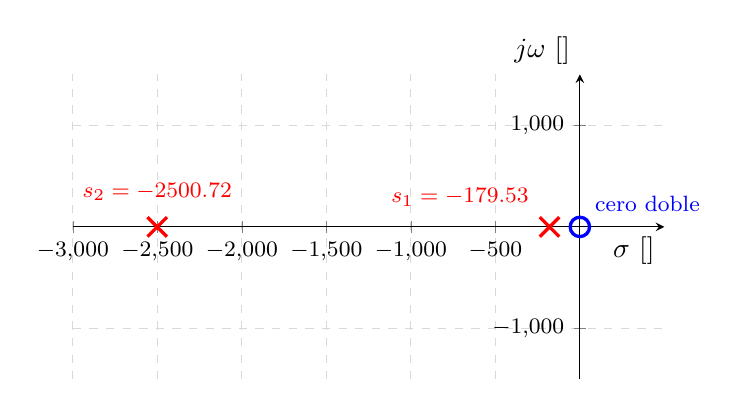
\begin{tikzpicture}
  \begin{axis}[
    width=0.75\textwidth, height=0.45\textwidth,
    axis lines=middle,
    xlabel={$\sigma$ [\unit{\radian\per\second}]},
    ylabel={$j\omega$ [\unit{\radian\per\second}]},
    xlabel style={at={(ticklabel* cs:1)}, anchor=north east},
    ylabel style={at={(ticklabel* cs:1)}, anchor=south east},
    xmin=-3000, xmax=500, ymin=-1500, ymax=1500,
    xtick={-3000,-2500,-2000,-1500,-1000,-500},
    ytick={-1000,1000},
    grid=both, grid style={gray!30, dashed},
    tick label style={font=\footnotesize},
    clip=false,
  ]
    \addplot[only marks, mark=x, mark size=5pt, very thick, red]
      coordinates {(-2500.72,0) (-179.53,0)};
    \addplot[only marks, mark=o, mark size=3.5pt, very thick, blue] coordinates {(0,0)};
    \node[above=6pt, red, font=\footnotesize] at (axis cs:-2500.72,0) {$s_2 = \num{-2500.72}$};
    \node[above left=4pt, red, font=\footnotesize] at (axis cs:-179.53,0) {$s_1 = \num{-179.53}$};
    \node[above right=2pt, blue, font=\footnotesize] at (axis cs:0,0) {cero doble};
  \end{axis}
\end{tikzpicture}
}}
      \vspace{3pt}
      \begin{tarjeta}[colframe=CardBorder, colback=CardBg, boxrule=0.5pt, top=3pt, bottom=3pt, left=5pt, right=5pt]
        {\fontsize{7.5pt}{9pt}\selectfont
        \textbf{\color{NavyDark} Dinámica Sobreamortiguada:} Dispersión de $14\times$ entre raíces ($s_1 = \mathbf{-179.5\ \text{rad/s}}$, $s_2 = -2500.7\ \text{rad/s}$). El polo lento $s_1$ gobierna el transitorio.
        }
      \end{tarjeta}
    \end{column}
  \end{columns}
\end{frame}

% SLIDE 12: Q=0.25 TEMPORAL
\begin{frame}
  \frametitle{Régimen Sobreamortiguado ($Q = 0.25$): Respuesta al Escalón}

  \begin{columns}[c, onlytextwidth]
    \begin{column}{0.44\textwidth}
      \begin{tarjeta}
        {\fontsize{9pt}{11pt}\selectfont \textbf{\color{NavyDark} Parámetros al Escalón Unitario:}}\\[2pt]
        {\fontsize{7.5pt}{9.2pt}\selectfont
        \[ v_o(t) = (1.0773 e^{-2500.7 t} - 0.0773 e^{-179.5 t}) u(t) \]
        \begin{itemize}\setlength{\itemsep}{2pt}
          \item \textbf{Valor inicial discontinuo:} $v_o(0^+) = \qty{1.0}{\volt}$.
          \item \textbf{Tiempo de caída ($\qty{90}{\percent}\to\qty{10}{\percent}$):} $\qty{0.70}{\milli\second}$.
          \item \textbf{Subpico máximo:} $\qty{-4.8}{\percent}$ (en $t = \qty{2.27}{\milli\second}$).
          \item \textbf{Tiempo de establecimiento ($\pm\qty{2}{\percent}$):}
          $t_s = \tau_1 \ln\left(\frac{0.0773}{0.02}\right) \approx \mathbf{\qty{7.53}{\milli\second}}$.
          \item Respuesta estrictamente aperiódica sin oscilación.
        \end{itemize}
        }
      \end{tarjeta}
    \end{column}

    \begin{column}{0.54\textwidth}
      \centering
      \adjustbox{max width=\linewidth, max height=3.6cm, keepaspectratio}{{\textwidth=16cm\begin{tikzpicture}
  \begin{axis}[
    name=principal,
    width=0.9\textwidth, height=0.55\textwidth,
    xlabel={$t$ [\unit{\milli\second}]}, ylabel={Tensión [\unit{\volt}]},
    xmin=0, xmax=12, ymin=-0.1, ymax=1.1,
    grid=both, grid style={gray!30, dashed},
    legend pos=north east, legend cell align=left, legend style={font=\footnotesize},
    tick label style={font=\footnotesize},
    samples=400, domain=0:12, no marks,
  ]
    \addplot[gray, thick, dotted] {1};
    \addlegendentry{$v_i(t)$ (escalón unitario)}
    \addplot[blue, very thick] {1.07734*exp(-2.50072*x) - 0.07734*exp(-0.17953*x)};
    \addlegendentry{$v_o(t)$ para $Q = \num{0.25}$}
    \addplot[red, dashed] {0.02};
    \addlegendentry{banda de $\pm\qty{2}{\percent}$}
    \addplot[red, dashed, forget plot] {-0.02};
    \draw[dashed, gray] (axis cs:7.53,-0.1) -- (axis cs:7.53,0.08);
  \end{axis}
  % detalle ampliado de la zona del subpico
  \begin{axis}[
    at={(principal.north east)}, anchor=north east, xshift=-0.6cm, yshift=-2.0cm,
    width=0.5\textwidth, height=0.28\textwidth,
    xmin=0, xmax=12, ymin=-0.07, ymax=0.04,
    ytick={-0.06,-0.04,-0.02,0,0.02},
    scaled y ticks=false,
    yticklabel style={/pgf/number format/fixed, /pgf/number format/precision=2},
    grid=both, grid style={gray!30, dashed},
    tick label style={font=\scriptsize},
    axis background/.style={fill=white},
    samples=400, domain=0:12, no marks,
  ]
    \addplot[blue, very thick] {1.07734*exp(-2.50072*x) - 0.07734*exp(-0.17953*x)};
    \addplot[red, dashed] {0.02};
    \addplot[red, dashed] {-0.02};
    \addplot[only marks, mark=*, mark size=1.5pt, black] coordinates {(2.269,-0.0478)};
    \node[below right=1pt, font=\scriptsize] at (axis cs:2.269,-0.0478)
      {subpico \qty{-4.8}{\percent} en $t = \qty{2.27}{\milli\second}$};
    \draw[dashed, gray] (axis cs:7.53,-0.07) -- (axis cs:7.53,0.04)
      node[pos=0.72, right, font=\scriptsize, black] {$t_s = \qty{7.53}{\milli\second}$};
    \node[anchor=north west, font=\scriptsize\itshape] at (rel axis cs:0.02,0.98) {detalle};
  \end{axis}
\end{tikzpicture}
}}
      \vspace{3pt}
      \begin{tarjeta}[colframe=CardBorder, colback=CardBg, boxrule=0.5pt, top=3pt, bottom=3pt, left=5pt, right=5pt]
        {\fontsize{7.5pt}{9pt}\selectfont
        \textbf{\color{NavyDark} Dinámica Aperiódica:} Respuesta estrictamente monótona sin oscilación. Subpico marginal de $\mathbf{-4.8\%}$ y establecimiento en $\mathbf{t_s = \qty{7.53}{\milli\second}}$.
        }
      \end{tarjeta}
    \end{column}
  \end{columns}
\end{frame}

% SLIDE 13: Q=0.75 POLOS
\subsection{Análisis Q = 0.75}
\begin{frame}
  \frametitle{Régimen Subamortiguado ($Q = 0.75$): Polos Complejos Conjugados}

  \begin{columns}[c, onlytextwidth]
    \begin{column}{0.46\textwidth}
      \begin{tarjeta}
        {\fontsize{9pt}{11pt}\selectfont \textbf{\color{NavyDark} Raíces Complejas en Plano s:}}\\[2pt]
        {\fontsize{7.5pt}{9.2pt}\selectfont
        \[ H_2(s) = \frac{s^2}{s^2 + 3542.33 s + 7056436} \]
        \begin{itemize}\setlength{\itemsep}{2pt}
          \item Con $\xi = 0.667 < 1$, discriminante negativo:
          $s_{1,2} = \mathbf{-1771.17 \pm j\, 1979.75\ \unit{\radian\per\second}}$.
          \item \textbf{Atenuación de envolvente:} $\sigma = \qty{1771.17}{\radian\per\second}$.
          \item \textbf{Pulsación amortiguada:}
          $\omega_d = \omega_0 \sqrt{1 - \xi^2} = \qty{1979.75}{\radian\per\second}$ ($f_d \approx \qty{315.1}{\hertz}$).
          \item Constante de envolvente: $\tau_2 = \mathbf{\qty{0.56}{\milli\second}}$ ($10\times$ más veloz).
        \end{itemize}
        }
      \end{tarjeta}
    \end{column}

    \begin{column}{0.52\textwidth}
      \centering
      \adjustbox{max width=\linewidth, max height=5.2cm, keepaspectratio}{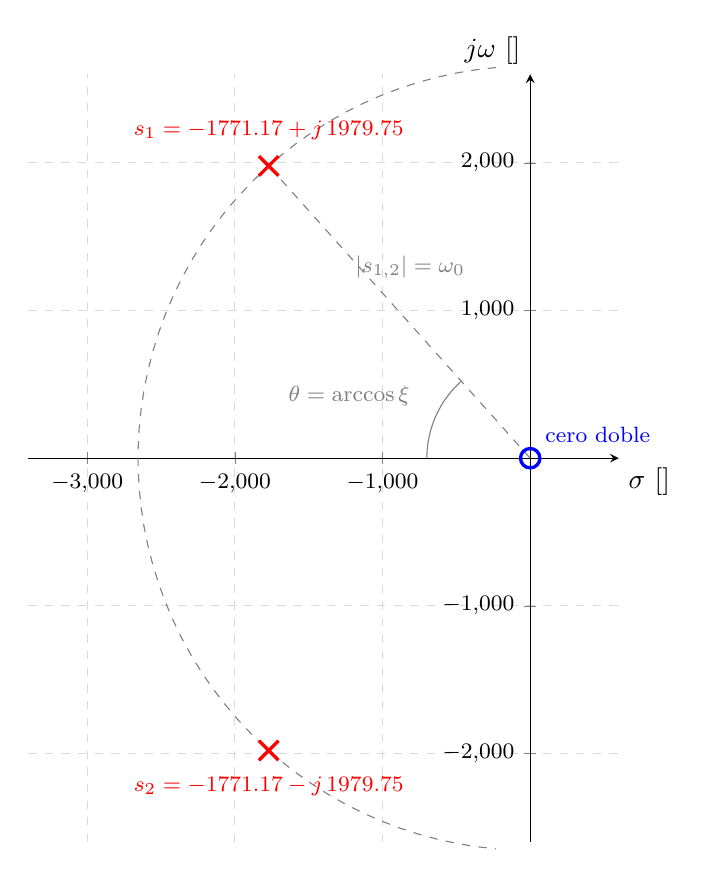
\begin{tikzpicture}
  \begin{axis}[
    % escala igual en ambos ejes: 4000 x 5200 rad/s sobre 7,5 cm x 9,75 cm
    scale only axis, width=7.5cm, height=9.75cm,
    axis lines=middle,
    xlabel={$\sigma$ [\unit{\radian\per\second}]},
    ylabel={$j\omega$ [\unit{\radian\per\second}]},
    xlabel style={at={(ticklabel* cs:1)}, anchor=north west},
    ylabel style={at={(ticklabel* cs:1)}, anchor=south east},
    xmin=-3400, xmax=600, ymin=-2600, ymax=2600,
    xtick={-3000,-2000,-1000},
    ytick={-2000,-1000,1000,2000},
    grid=both, grid style={gray!30, dashed},
    tick label style={font=\footnotesize},
    clip=false,
  ]
    % circunferencia de radio omega_0 sobre la que se ubican los polos
    \addplot[domain=95:265, samples=60, dashed, gray, no marks] ({2656.4*cos(x)}, {2656.4*sin(x)});
    \addplot[dashed, gray, no marks] coordinates {(0,0) (-1771.17,1979.75)};
    \addplot[domain=131.8:180, samples=20, gray, no marks] ({700*cos(x)}, {700*sin(x)});
    \addplot[only marks, mark=x, mark size=5pt, very thick, red]
      coordinates {(-1771.17,1979.75) (-1771.17,-1979.75)};
    \addplot[only marks, mark=o, mark size=3.5pt, very thick, blue] coordinates {(0,0)};
    \node[above=6pt, red, font=\footnotesize] at (axis cs:-1771.17,1979.75)
      {$s_1 = \num{-1771.17} + j\,\num{1979.75}$};
    \node[below=6pt, red, font=\footnotesize] at (axis cs:-1771.17,-1979.75)
      {$s_2 = \num{-1771.17} - j\,\num{1979.75}$};
    \node[above right=2pt, blue, font=\footnotesize] at (axis cs:0,0) {cero doble};
    \node[gray, font=\footnotesize, anchor=south west] at (axis cs:-1250,1150) {$|s_{1,2}| = \omega_0$};
    \node[gray, font=\footnotesize, anchor=east] at (axis cs:-750,420) {$\theta = \arccos\xi$};
  \end{axis}
\end{tikzpicture}
}
    \end{column}
  \end{columns}
\end{frame}

% SLIDE 14: Q=0.75 TEMPORAL
\begin{frame}
  \frametitle{Régimen Subamortiguado ($Q = 0.75$): Respuesta Temporal y Subpico}

  \begin{columns}[c, onlytextwidth]
    \begin{column}{0.45\textwidth}
      \begin{tarjeta}
        {\fontsize{8.5pt}{10pt}\selectfont \textbf{\color{NavyDark} Parámetros al Escalón Unitario:}}\\[2pt]
        {\fontsize{7pt}{8.5pt}\selectfont
        \[ v_o(t) = e^{-\sigma t} [\cos(\omega_d t) - 0.8946 \sin(\omega_d t)] u(t) \]
        \begin{itemize}\setlength{\itemsep}{1.5pt}
          \item $\sigma = \qty{1771.17}{\radian\per\second}, \quad \omega_d = \qty{1979.75}{\radian\per\second}$.
          \item \textbf{Valor inicial discontinuo:} $v_o(0^+) = \qty{1.0}{\volt}$.
          \item \textbf{Tiempo de caída ($\qty{90}{\percent}\to\qty{10}{\percent}$):} $\qty{0.33}{\milli\second}$ ($2.1\times$ más rápido).
          \item \textbf{Primer cruce por cero:} $t_0 = \qty{0.425}{\milli\second}$.
          \item \textbf{Subpico máximo:} $\mathbf{\qty{-22.2}{\percent}}$ (en $t = \qty{0.85}{\milli\second}$).
          \item \textbf{Tiempo de establecimiento ($\pm\qty{2}{\percent}$):}
          $t_s = \mathbf{\qty{1.82}{\milli\second}}$ ($4.1\times$ más rápido).
          \item \textbf{Período de oscilación:} $T_d = \frac{2\pi}{\omega_d} = \qty{3.17}{\milli\second}$.
        \end{itemize}
        }
      \end{tarjeta}
    \end{column}

    \begin{column}{0.53\textwidth}
      \centering
      \adjustbox{max width=\linewidth, max height=3.6cm, keepaspectratio}{{\textwidth=16cm\begin{tikzpicture}
  \begin{axis}[
    width=0.9\textwidth, height=0.5\textwidth,
    xlabel={$t$ [\unit{\milli\second}]}, ylabel={Tensión [\unit{\volt}]},
    xmin=0, xmax=4, ymin=-0.35, ymax=1.1,
    grid=both, grid style={gray!30, dashed},
    legend pos=north east, legend cell align=left, legend style={font=\footnotesize},
    tick label style={font=\footnotesize},
    samples=400, domain=0:4, no marks,
  ]
    \addplot[gray, thick, dotted] {1};
    \addlegendentry{$v_i(t)$ (escalón unitario)}
    \addplot[blue, very thick]
      {exp(-1.77117*x)*(cos(deg(1.97975*x)) - 0.8946*sin(deg(1.97975*x)))};
    \addlegendentry{$v_o(t)$ para $Q = \num{0.75}$}
    \addplot[orange, dashed, thick] {1.3416*exp(-1.77117*x)};
    \addlegendentry{envolvente $\pm\frac{\omega_0}{\omega_d}e^{-\sigma t}$}
    \addplot[orange, dashed, thick, forget plot] {-1.3416*exp(-1.77117*x)};
    \addplot[red, dashed] {0.02};
    \addlegendentry{banda de $\pm\qty{2}{\percent}$}
    \addplot[red, dashed, forget plot] {-0.02};
    \addplot[only marks, mark=*, mark size=1.8pt, black, forget plot] coordinates {(0.850,-0.222)};
    \node[below right=2pt, font=\footnotesize] at (axis cs:0.850,-0.222)
      {subpico \qty{-22.2}{\percent} en $t = \qty{0.85}{\milli\second}$};
    \addplot[only marks, mark=*, mark size=1.8pt, black, forget plot] coordinates {(0.425,0)};
    \node[above right=2pt, font=\footnotesize] at (axis cs:0.425,0) {$t = \qty{0.425}{\milli\second}$};
    \draw[dashed, gray] (axis cs:1.82,-0.35) -- (axis cs:1.82,0.5)
      node[pos=1, above, font=\footnotesize, black] {$t_s = \qty{1.82}{\milli\second}$};
  \end{axis}
\end{tikzpicture}
}}
      \vspace{3pt}
      \begin{tarjeta}[colframe=CardBorder, colback=CardBg, boxrule=0.5pt, top=3pt, bottom=3pt, left=5pt, right=5pt]
        {\fontsize{7.5pt}{9pt}\selectfont
        \textbf{\color{AlertAmber} Dinámica Rápida Subamortiguada:} Recuperación en solo $\mathbf{t_s = \qty{1.82}{\milli\second}}$ ($4.1\times$ más veloz que $Q=0.25$) a costa de un subpico del $\mathbf{-22.2\%}$.
        }
      \end{tarjeta}
    \end{column}
  \end{columns}
\end{frame}

% SLIDE 15: COMPARATIVA TEMPORAL
\subsection{Comparativa Temporal}
\begin{frame}
  \frametitle{Comparativa Temporal Directa: $Q = 0.25$ vs $Q = 0.75$}

  \begin{columns}[c, onlytextwidth]
    \begin{column}{0.48\textwidth}
      \centering
      \adjustbox{max width=\linewidth, max height=3.5cm, keepaspectratio}{{\textwidth=16cm\begin{tikzpicture}
  \begin{axis}[
    width=0.9\textwidth, height=0.5\textwidth,
    xlabel={$t$ [\unit{\milli\second}]}, ylabel={$v_o(t)$ [\unit{\volt}]},
    xmin=0, xmax=8, ymin=-0.3, ymax=1.05,
    grid=both, grid style={gray!30, dashed},
    legend pos=north east, legend cell align=left, legend style={font=\footnotesize},
    tick label style={font=\footnotesize},
    samples=400, domain=0:8, no marks,
  ]
    \addplot[blue, very thick] {1.07734*exp(-2.50072*x) - 0.07734*exp(-0.17953*x)};
    \addlegendentry{$Q = \num{0.25}$ ($\xi = 2$, sobreamortiguado)}
    \addplot[red!80!black, very thick]
      {exp(-1.77117*x)*(cos(deg(1.97975*x)) - 0.8946*sin(deg(1.97975*x)))};
    \addlegendentry{$Q = \num{0.75}$ ($\xi = \num{0.667}$, subamortiguado)}
    \addplot[gray, dashed] {0.02};
    \addlegendentry{banda de $\pm\qty{2}{\percent}$}
    \addplot[gray, dashed, forget plot] {-0.02};
  \end{axis}
\end{tikzpicture}
}}
      \vspace{3pt}
      \begin{tarjeta}[colframe=CardBorder, colback=CardBg, boxrule=0.5pt, top=3pt, bottom=3pt, left=5pt, right=5pt]
        {\fontsize{7.5pt}{9pt}\selectfont
        \textbf{\color{NavyDark} Compromiso Fundamental:} $Q=0.75$ prioriza velocidad ($1.82\text{ ms}$) con oscilación; $Q=0.25$ asegura monotonía ($7.53\text{ ms}$) sin sobreimpulsos.
        }
      \end{tarjeta}
    \end{column}

    \begin{column}{0.50\textwidth}
      \begin{tarjeta}
        {\fontsize{8.5pt}{10pt}\selectfont \textbf{\color{NavyDark} Comparación de Parámetros Temporales:}}\\[2pt]
        \resizebox{\linewidth}{!}{%
        \setlength{\tabcolsep}{3pt}
        \renewcommand{\arraystretch}{1.05}
        {\fontsize{7pt}{8.5pt}\selectfont
        \begin{tabular}{lcc}
          \toprule
          \textbf{Parámetro} & \textbf{$Q = 0.25$} & \textbf{$Q = 0.75$} \\
          \midrule
          Factor amortiguamiento $\xi$ & $2.000$ & $0.667$ \\
          Tipo de amortiguamiento & Sobreamortiguado & Subamortiguado \\
          Raíces en plano $s$ & $-179.5\ ;\ -2500.7$ & $-1771.2 \pm j 1979.8$ \\
          Tiempo caída ($\qty{90}{\percent}\to\qty{10}{\percent}$) & $\qty{0.70}{\milli\second}$ & $\qty{0.33}{\milli\second}$ \\
          Subpico máximo & $\mathbf{-4.8\%}$ & $\mathbf{-22.2\%}$ \\
          Tiempo establecimiento ($2\%$) & $\qty{7.53}{\milli\second}$ & $\mathbf{\qty{1.82}{\milli\second}}$ \\
          Inductancia $L$ & $\qty{37.31}{\milli\henry}$ & $\qty{28.23}{\milli\henry}$ \\
          Capacidad $C$ & $\qty{59.70}{\micro\farad}$ & $\qty{5.02}{\micro\farad}$ \\
          \bottomrule
        \end{tabular}
        }%
        }
      \end{tarjeta}
    \end{column}
  \end{columns}
\end{frame}

% SLIDE 16: COMPARATIVA FRECUENCIAL
\subsection{Comparativa Frecuencial}
\begin{frame}
  \frametitle{Comparativa Frecuencial Directa: $Q = 0.25$ vs $Q = 0.75$}

  \begin{columns}[c, onlytextwidth]
    \begin{column}{0.56\textwidth}
      \centering
      \adjustbox{max width=\linewidth, max height=4.8cm, keepaspectratio}{{\textwidth=16cm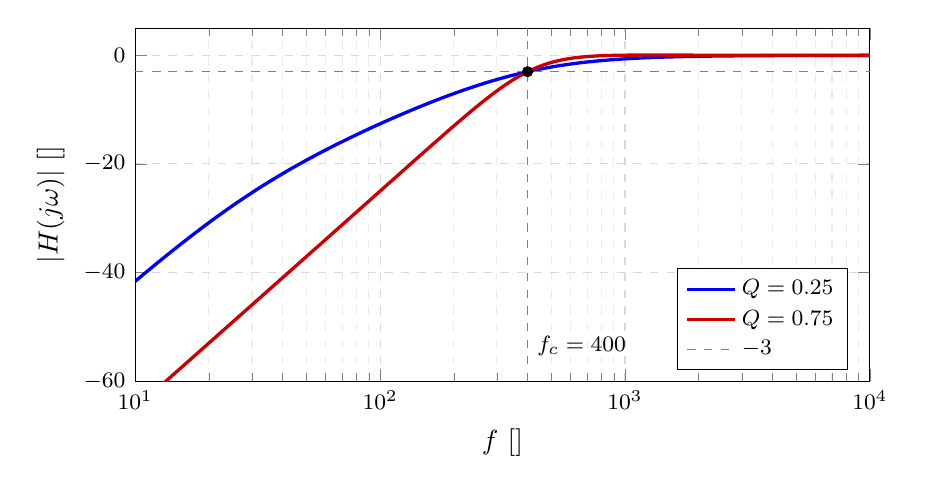
\begin{tikzpicture}
  \begin{semilogxaxis}[
    width=0.9\textwidth, height=0.5\textwidth,
    xlabel={$f$ [\unit{\hertz}]}, ylabel={$|H(j\omega)|$ [\unit{\decibel}]},
    xmin=10, xmax=10000, ymin=-60, ymax=5,
    grid=both, grid style={gray!30, dashed},
    minor grid style={gray!15, dashed},
    legend pos=south east, legend cell align=left, legend style={font=\footnotesize},
    tick label style={font=\footnotesize},
    samples=150, domain=10:10000, no marks,
  ]
    \addplot[blue, very thick]
      {20*log10((2*pi*x)^2 / sqrt((670.04^2 - (2*pi*x)^2)^2 + (670.04*2*pi*x/0.25)^2))};
    \addlegendentry{$Q = \num{0.25}$}
    \addplot[red!80!black, very thick]
      {20*log10((2*pi*x)^2 / sqrt((2656.40^2 - (2*pi*x)^2)^2 + (2656.40*2*pi*x/0.75)^2))};
    \addlegendentry{$Q = \num{0.75}$}
    \addplot[gray, dashed] {-3.01};
    \addlegendentry{$\qty{-3}{\decibel}$}
    \draw[dashed, gray] (axis cs:400,-60) -- (axis cs:400,5)
      node[pos=0.1, right, font=\footnotesize, black] {$f_c = \qty{400}{\hertz}$};
    \addplot[only marks, mark=*, mark size=1.8pt, black, forget plot] coordinates {(400,-3.01)};
  \end{semilogxaxis}
\end{tikzpicture}
}}
    \end{column}

    \begin{column}{0.42\textwidth}
      \begin{tarjeta}
        {\fontsize{8.5pt}{10.5pt}\selectfont \textbf{\color{NavyDark} Contraste en Diagrama de Bode:}}\\[2pt]
        {\fontsize{7.5pt}{9.2pt}\selectfont
        \begin{itemize}\setlength{\itemsep}{2pt}
          \item \textbf{Pasa alto con $Q_1 = 0.25$:}
          Rodilla de transición muy suave y redondeada. Atenuación prematura en la cercanía de la banda de paso.
          \item \textbf{Pasa alto con $Q_2 = 0.75$:}
          Transición abrupta y selectiva en torno a $f_c = \qty{400}{\hertz}$. Mantiene mayor ganancia en banda útil.
          \item \textbf{Conclusión de diseño:}
          $Q=0.25$ es mandatorio ante tolerancia nula a oscilaciones; $Q=0.75$ es superior para filtrado rápido y selectivo.
        \end{itemize}
        }
      \end{tarjeta}
    \end{column}
  \end{columns}
\end{frame}
